\section{Reálné snímky}
\label{sec:Chapter64}
Při zpracovávání manuálně vytvořených reálných snímcích jsme došli k několika zjištěním. Sítě selžou v úloze lokalizace při představení náhodných změn v pohledu. Poté zase můžeme pozorovat zlepšení sítě U-Net++ bez HS (snímek \ref{fig:real_unet_ppa}) oproti síti U-Net (snímek \ref{fig:real_unet_a}). Ve středovém snímku proběhla úspěšná lokalizace, na krajních dvou neproběhla. Příčinou může být větší počet parametrů sítě. U sítí U-Net STN se klíčový bod nepovedlo také lokalizovat.
\begin{figure}[H]
\centering

\newcommand{\subfiguresize}{.15\textwidth}
\newcommand{\imagewidth}{1.0in}
\newcommand{\hspacesize}{.00in}

\newcommand{\insertimage}[1]{%
  \begin{minipage}{\imagewidth}
    \centering
    \includegraphics[width=\imagewidth]{#1}
  \end{minipage}
}

\subfloat[]{%
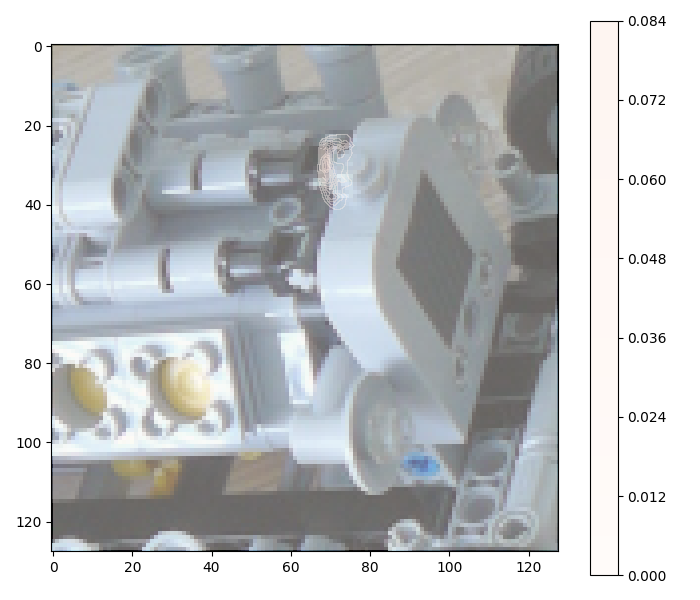
\includegraphics[width=0.32\textwidth,keepaspectratio]{Figures/real_n_pp/a0.png}
}\hspace{\hspacesize}%
\subfloat[]{%
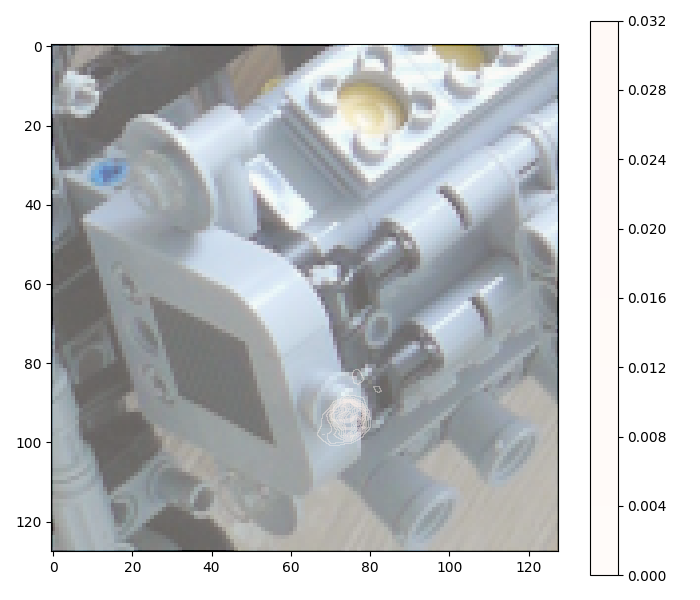
\includegraphics[width=0.32\textwidth,keepaspectratio]{Figures/real_n_pp/a1.png}
}\hspace{\hspacesize}%
\subfloat[]{%
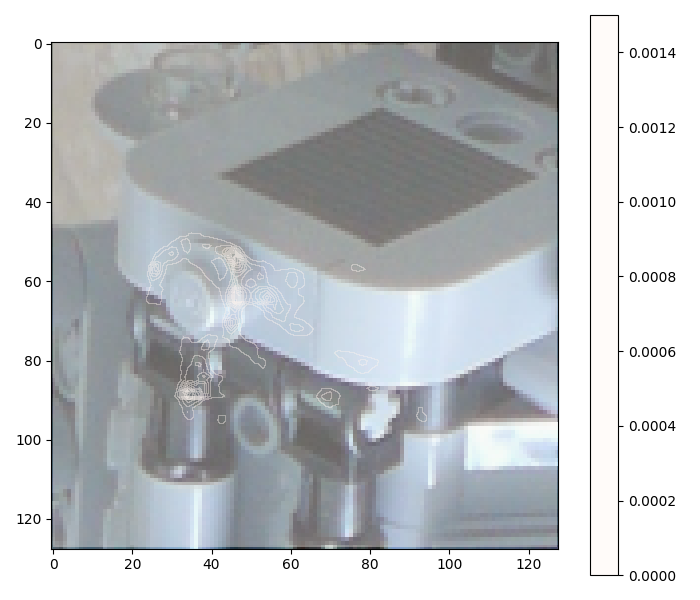
\includegraphics[width=0.32\textwidth,keepaspectratio]{Figures/real_n_pp/a2.png}
}
\caption[Reálné snímky zpracované sítí U-Net]
{Reálné snímky zpracované sítí U-Net pro klíčový bod č. 0. }
\label{fig:real_unet_a}
\end{figure}


\begin{figure}[H]
\centering

\newcommand{\subfiguresize}{.15\textwidth}
\newcommand{\imagewidth}{1.0in}
\newcommand{\hspacesize}{.00in}

\newcommand{\insertimage}[1]{%
  \begin{minipage}{\imagewidth}
    \centering
    \includegraphics[width=\imagewidth]{#1}
  \end{minipage}
}

\subfloat[]{%
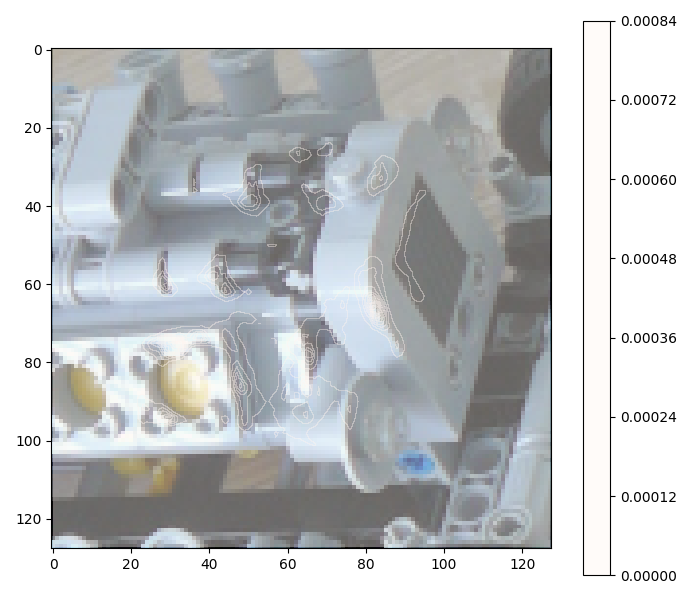
\includegraphics[width=0.32\textwidth,keepaspectratio]{Figures/real_n_pp/ppa0.png}
}\hspace{\hspacesize}%
\subfloat[]{%
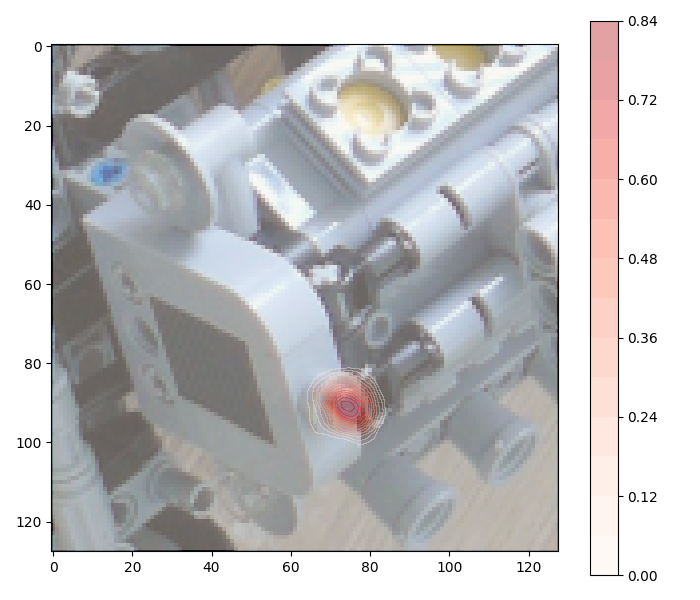
\includegraphics[width=0.32\textwidth,keepaspectratio]{Figures/real_n_pp/ppa1.png}
}\hspace{\hspacesize}%
\subfloat[]{%
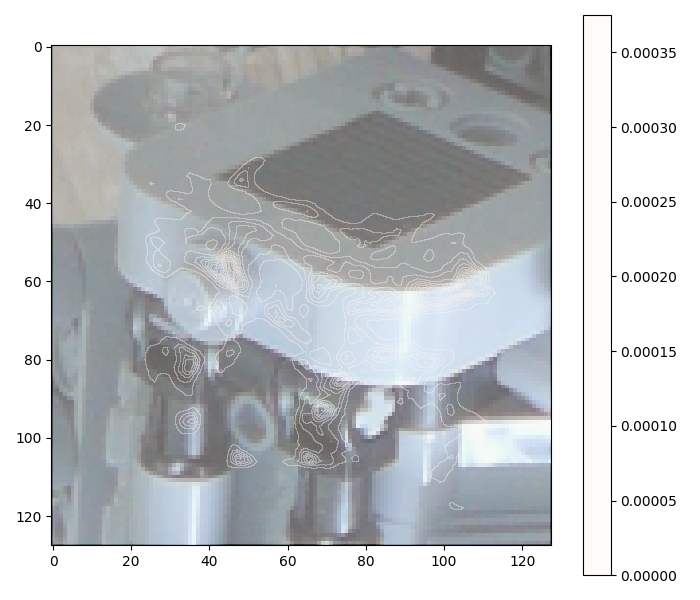
\includegraphics[width=0.32\textwidth,keepaspectratio]{Figures/real_n_pp/ppa2.png}
}
\caption[Reálné snímky zpracované sítí U-Net++ bez HS]
{Reálné snímky zpracované sítí U-Net++ bez HS pro klíčový bod č. 0}
\label{fig:real_unet_ppa}
\end{figure}

V následujícím případě se povedlo všem sítím podobně lokalizovat klíčový bod č. 2 (snímek \ref{fig:real_unet_stn}):

\begin{figure}[H]
\centering

\newcommand{\subfiguresize}{.15\textwidth}
\newcommand{\imagewidth}{1.0in}
\newcommand{\hspacesize}{.00in}

\newcommand{\insertimage}[1]{%
  \begin{minipage}{\imagewidth}
    \centering
    \includegraphics[width=\imagewidth]{#1}
  \end{minipage}
}

\subfloat[]{%
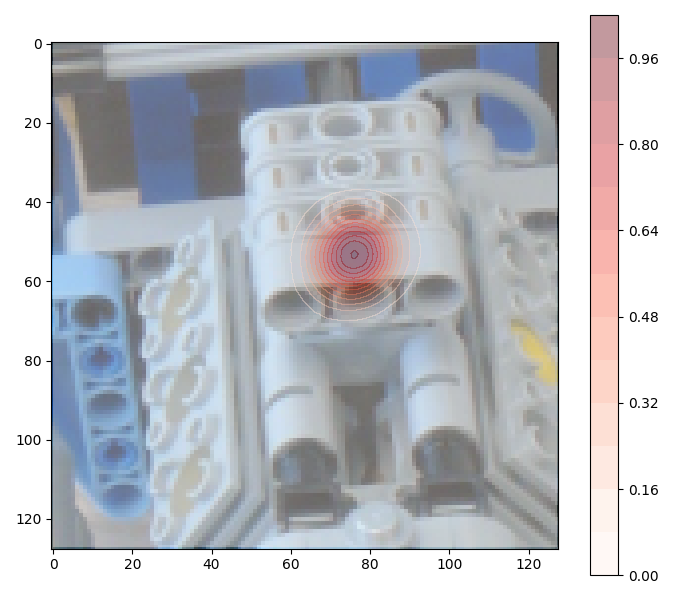
\includegraphics[width=0.32\textwidth,keepaspectratio]{Figures/real/b0.png}
}\hspace{\hspacesize}%
\subfloat[]{%
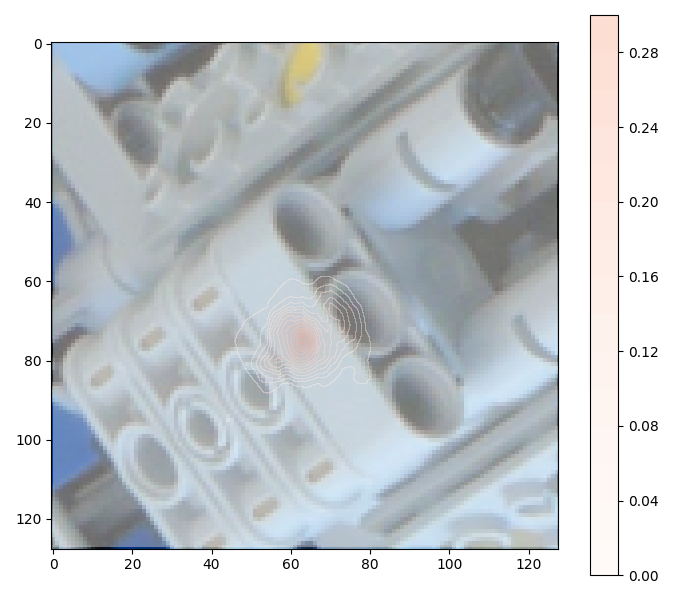
\includegraphics[width=0.32\textwidth,keepaspectratio]{Figures/real/b1.png}
}\hspace{\hspacesize}%
\subfloat[]{%
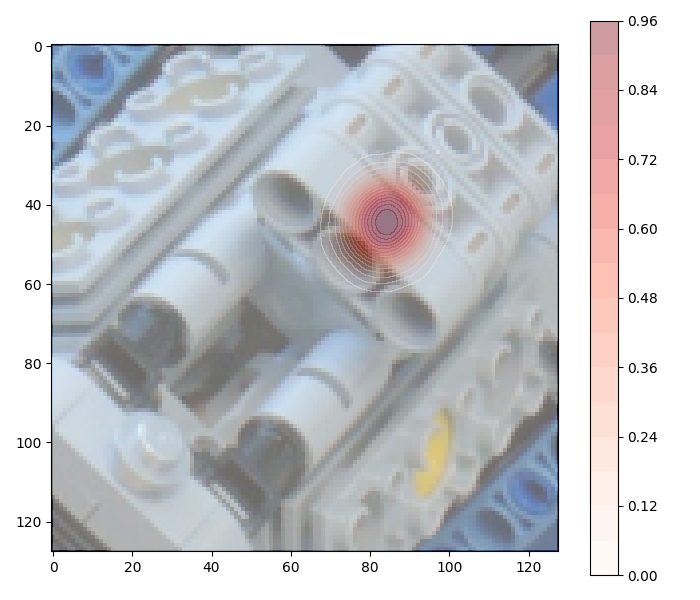
\includegraphics[width=0.32\textwidth,keepaspectratio]{Figures/real/b2.png}
}
\caption[Reálné snímky zpracované sítí U-Net STN 6p]
{Reálné snímky zpracované sítí U-Net STN s 6 parametry pro klíčový bod č. 2}
\label{fig:real_unet_stn}
\end{figure}


\begin{figure}[ht]
\centering
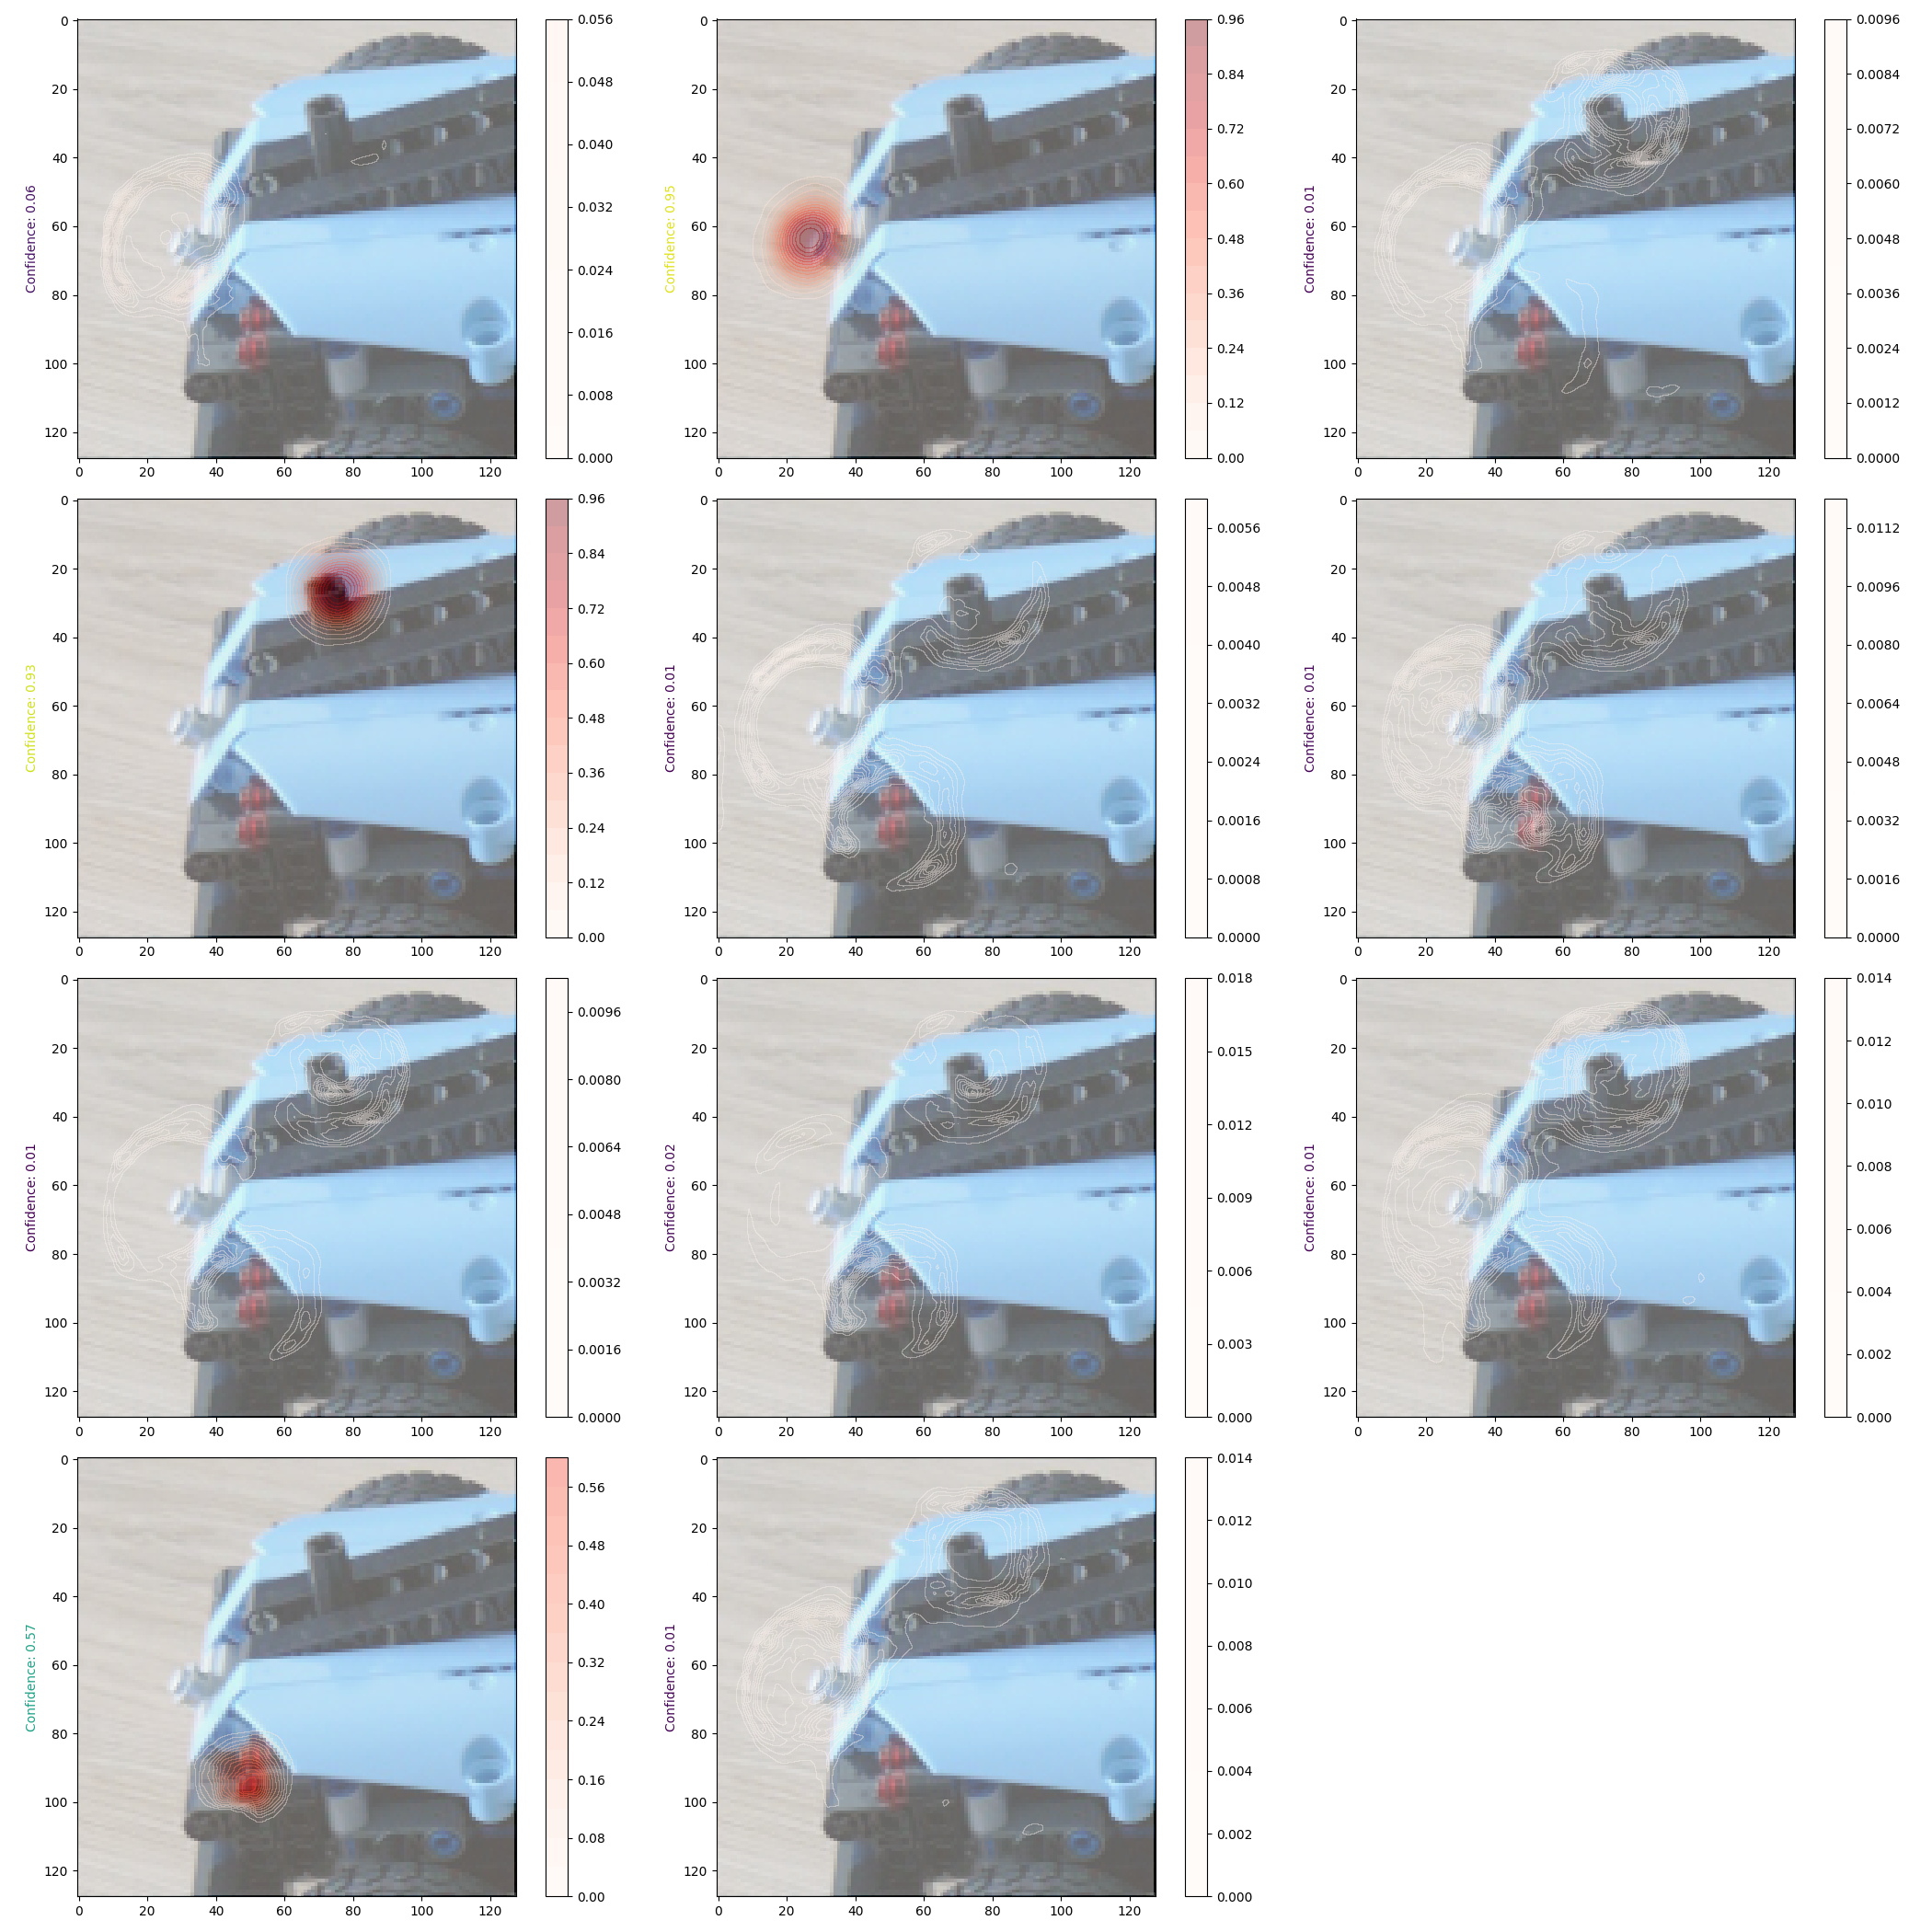
\includegraphics[width=1.0\textwidth,keepaspectratio]{Figures/real/real_3.png}
\caption[Demonstrace U-Net STN 6p na reálném snímku]{Demonstrace U-Net STN s 6 parametry na reálném snímku pro všech 11 kanálů. Výstupní skalární pole je transformováno na původní souřadnice snímku.}
\label{fig:real_0}
\end{figure}

Je zřejmé, že schopnosti prostorové invariance nebylo dosaženo do stavu, ve kterém by sítě byly konzistentně schopny odolávat všem změnám pohledu. Všechny sítě vykazují skvělé schopnosti na testovacím datasetu, avšak výsledky reálných snímků jsou při manuálních editacích podmíněny konkrétními pohledy. Očekávaná korektní lokalizace může být zobrazena na obrázku \ref{fig:real_0} pomocí sítě U-Net STN s 6 parametry.

\subsection{Demonstrace DINOv2}

Pomocí nástroje dle repozitáře \cite{jupyter_sparse_matching} postaveném na základě knihovny PyTorch byl v rámci této práce také implementován příklad detekce a korespondence klíčových bodů dle tzv. sparse matching sítě DINOv2. K tomu jsme využili dva neupravené reálné snímky a manuálně vytvořené masky (obrázek \ref{fig:dinov2_mask}). Detekce a korespondence na dvou reálných snímcích modelu LEGO auta lze vidět na obrázku \ref{fig:dinov2_sparse_car_lego}.

\begin{figure}[H]
\centering

\newcommand{\subfiguresize}{.15\textwidth}
\newcommand{\imagewidth}{1.0in}
\newcommand{\hspacesize}{.00in}

\newcommand{\insertimage}[1]{%
  \begin{minipage}{\imagewidth}
    \centering
    \includegraphics[width=\imagewidth]{#1}
  \end{minipage}
}

\subfloat[Snímek auta]{%
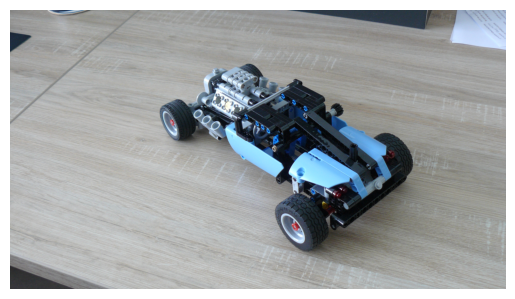
\includegraphics[width=0.32\textwidth,keepaspectratio]{Figures/dinov2/dinov2_raw.png}
  \label{fig:dinov2_raw}%
}\hspace{\hspacesize}%
\subfloat[Maska pro snímek auta]{%

\includegraphics[width=0.32\textwidth,keepaspectratio]{Figures/dinov2/dinov2_mask.png}
  \label{fig:dinov2_mask}%
}\hspace{\hspacesize}%
\subfloat[Extrahované příznaky sítí DINOv2]{%
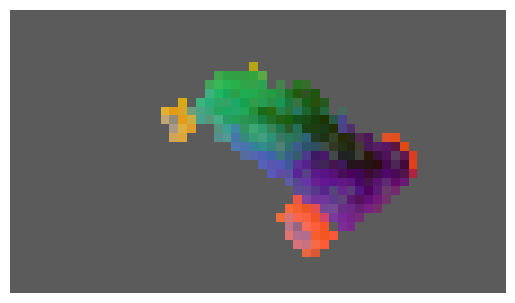
\includegraphics[width=0.32\textwidth,keepaspectratio]{Figures/dinov2/dinov2_vis.png}
  \label{fig:dinov2_vis}%
}
\caption[Snímek, maska a extrahované příznaky pro DINOv2]
{Snímek, maska a extrahované příznaky pro DINOv2. Snímek a maska jsou vstupem do sítě DINOv2. }
\label{fig:dinov2_masks}
\end{figure}

\begin{figure}[H]
\centering
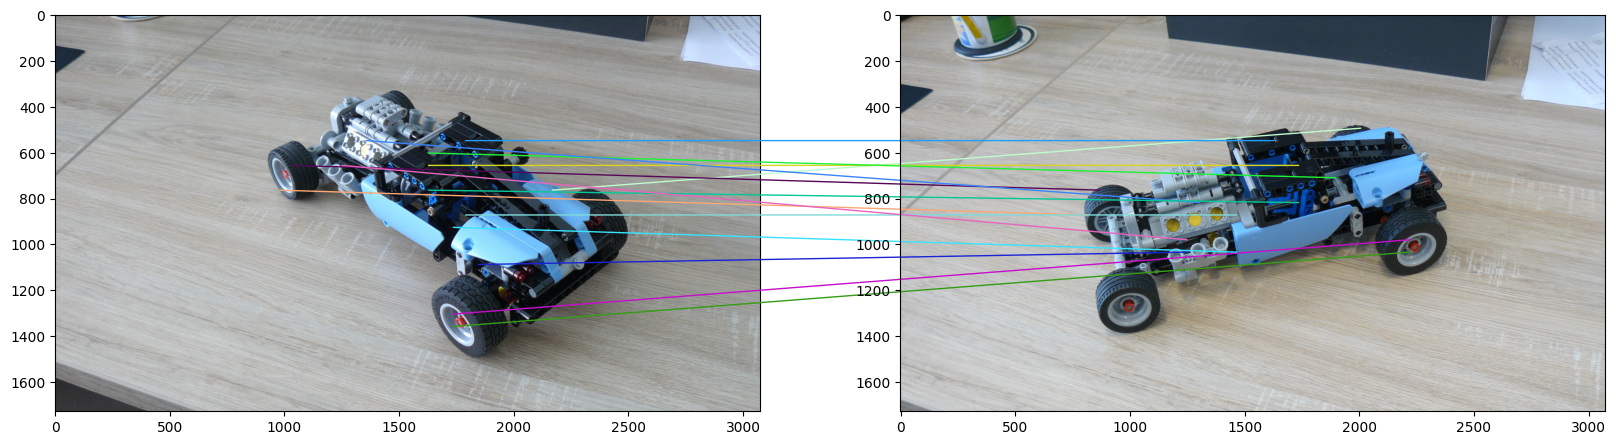
\includegraphics[width=1.0\textwidth,keepaspectratio]{Figures/dinov2demo.png}
\caption[Demonstrace tzv. sparse matching sítě DINOv2]{Demonstrace tzv. sparse matching sítě DINOv2. Síť se s pomocí vstupních obrazů a relevantních masek pokouší provést lokalizaci a korespondenci mezi klíčovými body na modelu auta.}
\label{fig:dinov2_sparse_car_lego}
\end{figure}

\begin{figure}[H]
\centering
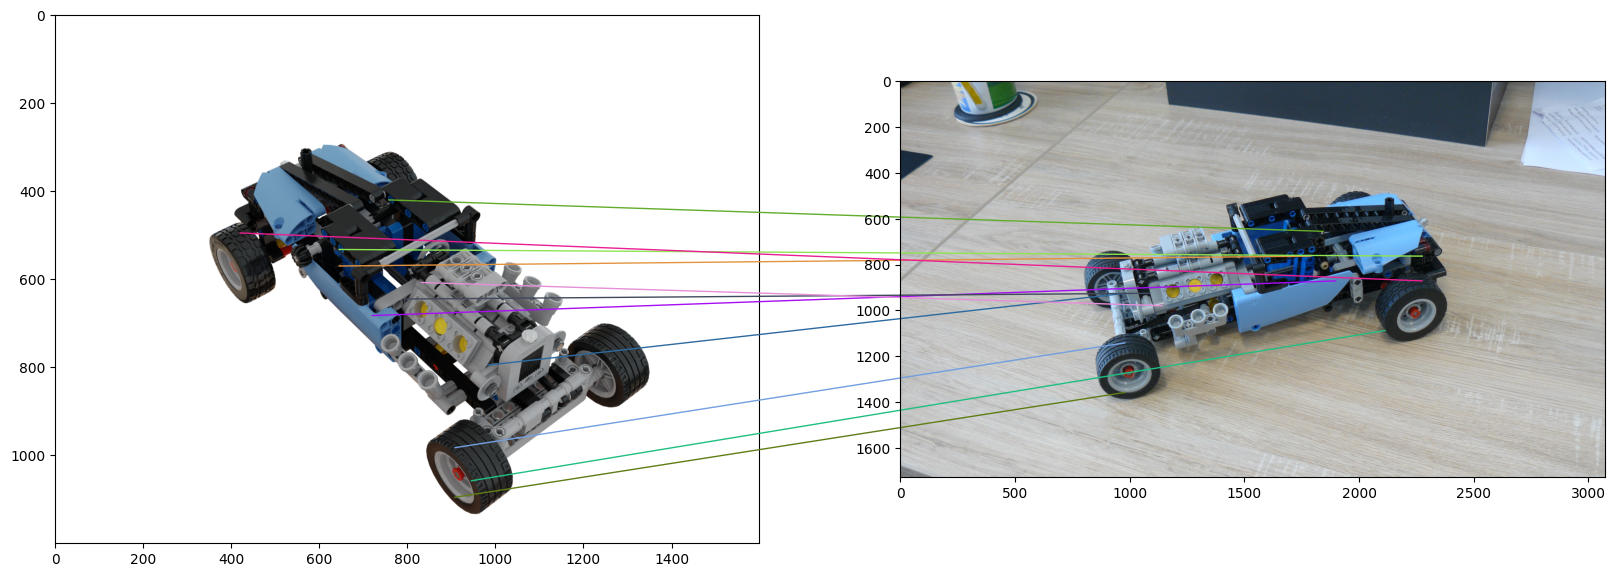
\includegraphics[width=1.0\textwidth,keepaspectratio]{Figures/dinov2/dinov2_synth.png}
\caption[Demonstrace tzv. sparse matching sítě DINOv2 na syntetickém snímku]{Demonstrace tzv. sparse matching sítě DINOv2 mezi syntetickým snímkem a reálným snímkem }
\label{fig:dinov2_sparse_synthetic}
\end{figure}
\endinput